\documentclass{article}
\usepackage[landscape, margin=0cm, paperheight=21cm, paperwidth=21cm]{geometry}
\usepackage{nopageno}
\usepackage{ifthen}
\usepackage{tikz}
\usepackage{fix-cm}


% CONFIGURABLE OPTIONS 
%
% The following *positive integer* specifies how large a box should
% be.
\def\totaldimension{10}
% The following specifies the font style
\def\letterfont{\fontsize{130}{0}\ttfamily\selectfont}
% The following specifies the arrow color
\def\arrowcolor{orange}
% The following specifies other arrow properties
\def\arrowheadstyle{latex}
\def\arrowlinewidth{10pt}
% The following number controls the opacity of the first arrow.
% Should be a number real number x in [0,1].
\def\startingopacity{1}
% The following controls the fill color of the initial and final
% cells.
\tikzstyle{initialcellstyle} = [fill=green!50, draw=black, opacity=.5]
\tikzstyle{finalcellstyle} = [fill=red!50, draw=black, opacity=.5]
% Uncomment if you want to see debug grids
%\newcommand{\debugme}{}


%---------------------------------------------------------------
% Do not touch the following unless you know what you are doing.
%---------------------------------------------------------------
\def\topx{-\totaldimension}
\def\topy{\totaldimension}
\def\botx{\totaldimension}
\def\boty{-\totaldimension}
\newcounter{boardindex}
\providecommand{\StartX}{0}
\providecommand{\StartY}{0}
\newcommand{\drawone}[2]{\draw (#1, #2) node {\usebox{\one}};}
\newcommand{\drawnegone}[2]{\draw (#1, #2) node {\usebox{\negone}};}
\newcommand{\drawthree}[2]{\draw (#1, #2) node {\usebox{\three}};}
\newcommand{\drawnegthree}[2]{\draw (#1, #2) node {\usebox{\negthree}};}
\newcommand{\drawfour}[2]{\draw (#1, #2) node {\usebox{\four}};}
\newcommand{\drawnegfour}[2]{\draw (#1, #2) node {\usebox{\negfour}};}
\newcommand{\drawfive}[2]{\draw (#1, #2) node {\usebox{\five}};}
\newcommand{\drawnegfive}[2]{\draw (#1, #2) node {\usebox{\negfive}};}
\newcommand{\drawinitialcell}[2]{\draw (#1, #2) node {\usebox{\initcell}};}
\newcommand{\drawfinalcell}[2]{\draw (#1, #2) node {\usebox{\finalcell}};}
% Cell dimension is the height/width of each cell
% in centimeters. It is given by
% min (floor((botx - topx)/4), floor((topy - boty)/4)
\def\celldimension{5}
%---------------------------------------------------------------
% Do not touch the above unless you know what you are doing.
%---------------------------------------------------------------

% These are fallback definitions.  When drawing a board, the following
% must be specified as "arguments":
% 
% \BOARD -- the game board, an array of 16 strings.  
%
% \LOCAT -- an array of numbers in the order which the board will be
% traversed
%
% \LISTLENGTH -- a single number equal to [length(LOCAT) - 2];
\providecommand{\BOARD}{{"A","B","C","D","E","F","G","H","I","J","K","L","M","N","O","P"}}
\providecommand{\drawarrows}{\drawone{0}{0}\drawinitialcell{0}{0}}

%% Start producing this way.
\providecommand{\PRODUCEPAGE}{\begin{center}
\begin{tikzpicture}
  % Draw the board.
  \node[inner sep=0pt] {\usebox{\gameboard}};

  % Draw arrows.
  \drawarrows
\end{tikzpicture}
\end{center}
}
\providecommand{\PRODUCEDOCUMENT}{\PRODUCEPAGE}


\begin{document}
\newsavebox{\gameboard}
\savebox{\gameboard}{
  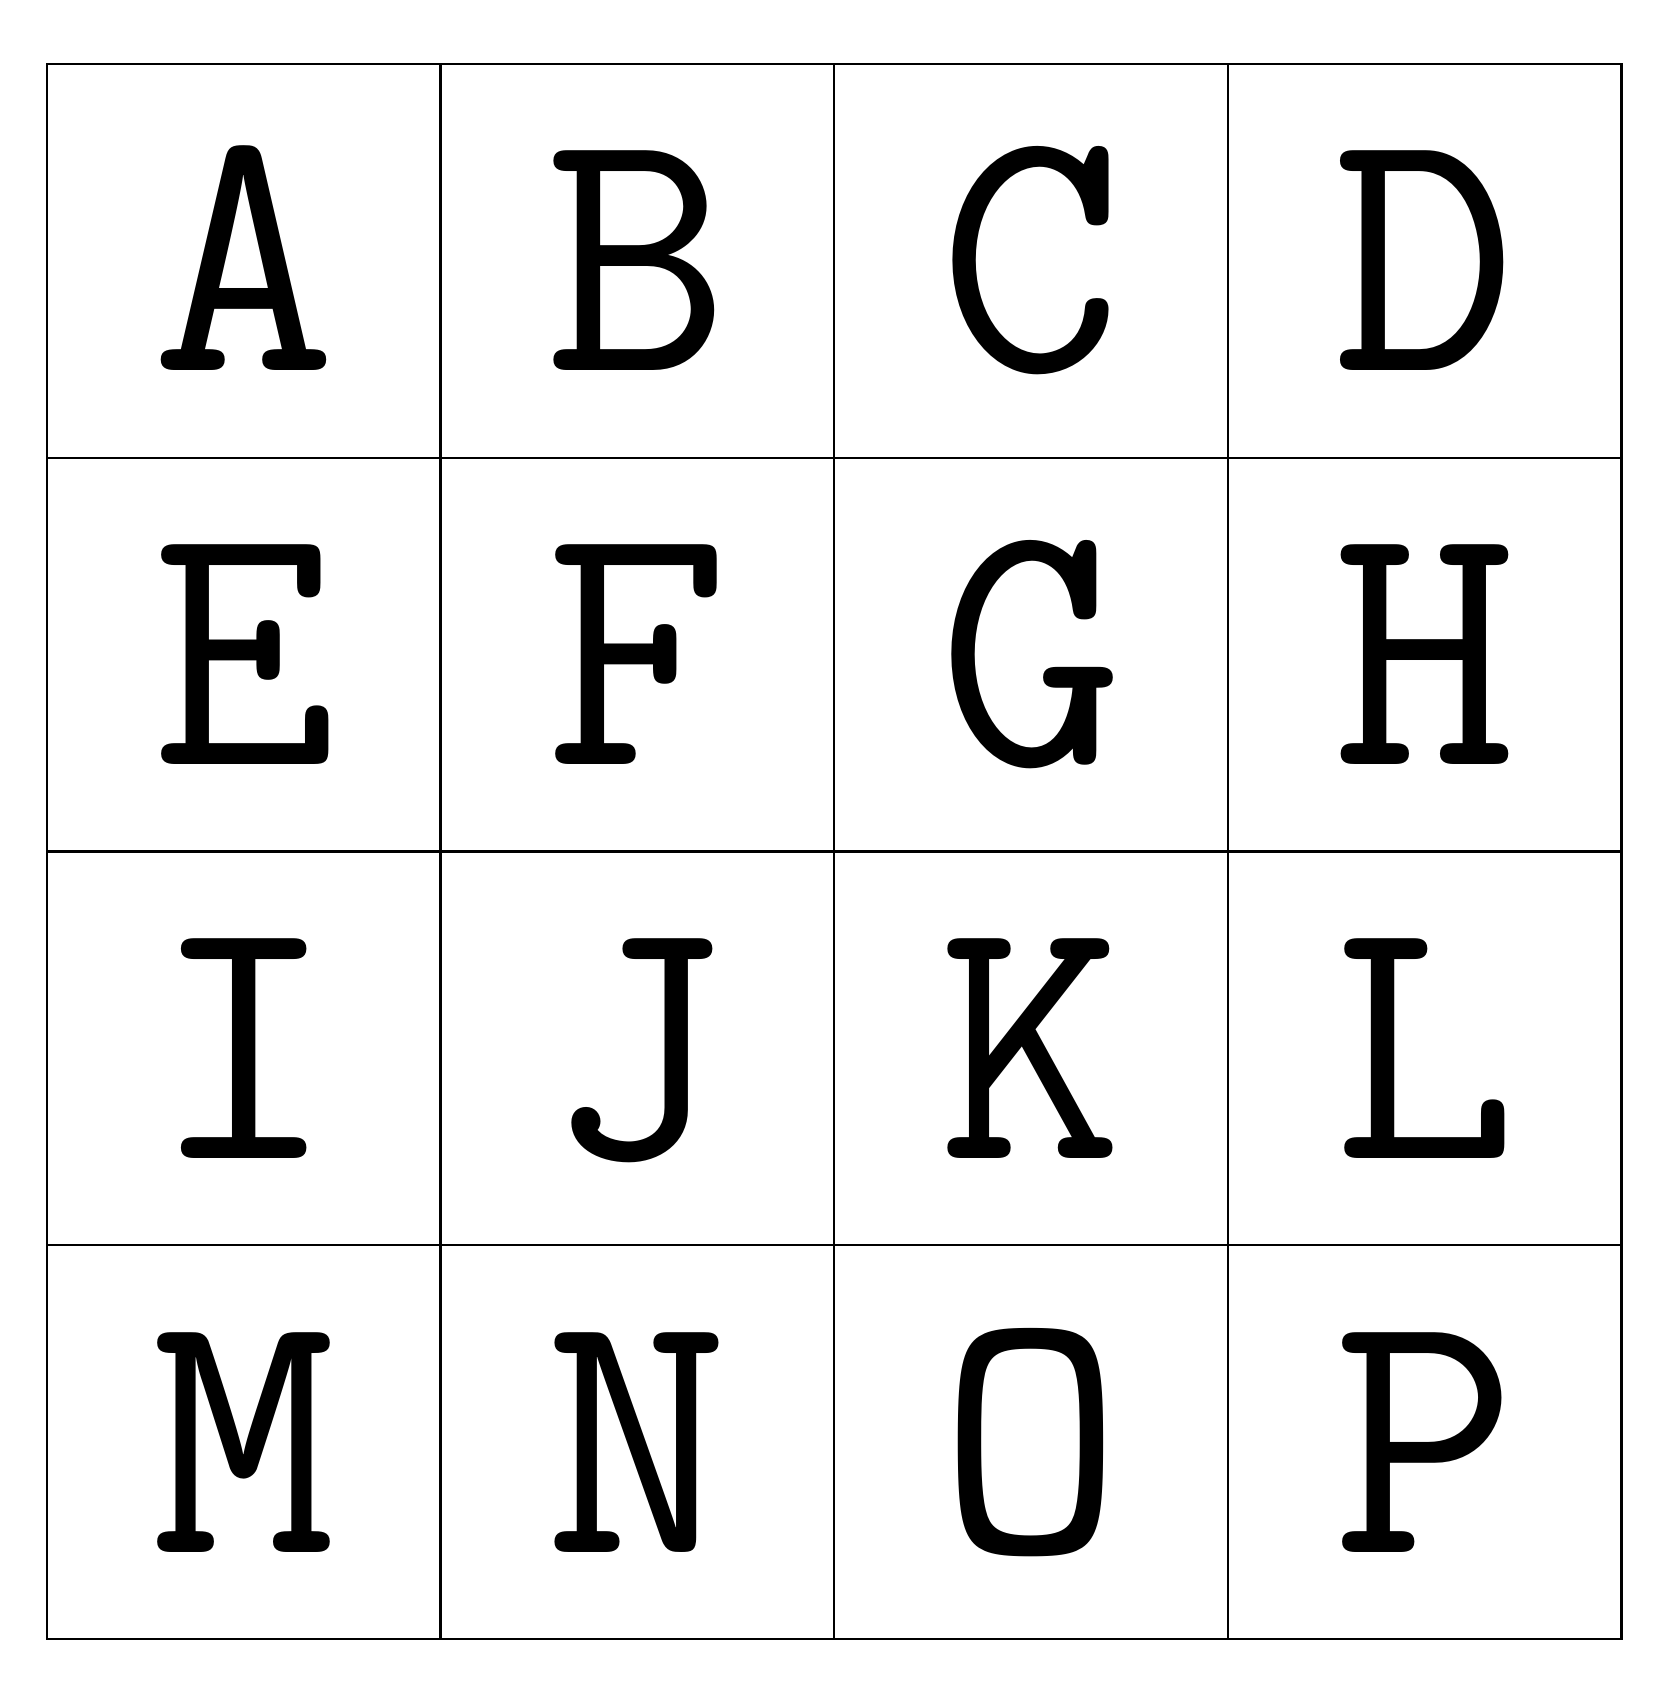
\begin{tikzpicture}[thick,scale=1]
    \setcounter{boardindex}{0}
    % Here we first draw a grid to help us debug.
    % The grid is drawn here:
    \ifthenelse{\isundefined{\debugme}}
    {}
    {\draw[step=1cm,gray,very thin] (-10,-10) grid (10,10);}

    % Cartesian coordinates are added here:
    \ifthenelse{\isundefined{\debugme}}
    {}
    {
    \foreach \x in {-9,...,9}
    \foreach \y in {-9,...,9}
    {
      \draw (\x, \y) node {{\tiny (\x, \y)}};
    }
    }
    
    % Calculate the dimensions of each square. 
    % We need to draw a 4x4 tableau, such that it is
    % horizontally and vertically centered at
    % the origin, and such that the each cell in
    % tableau is as large as possible.
    %
    % We require each cell to have an integral
    % dimension. Thus, the dimension is equal to
    % celldimension = 
    % min( floor( (\botx - \topx)/4 ), floor( (\topy - \boty)/4 ))
    
    % Uncomment below to regenerate ....
    % +++++++++++++++++++++++++++++++++++
    %\pgfmathparse{min( floor( (\botx - \topx)/4 ), floor( (\topy -
    %  \boty)/4 ))};
    %\let\celldimension\pgfmathresult
    % +++++++++++++++++++++++++++++++++++
    

    % Now we draw the tableau, starting at
    % top left = (-2 * \celldimension, 2 * \celldimension)
    % and ending at
    % bottom right = (2 * \celldimension, -2 * \celldimension)

    % We loop unroll instead to make this faster.
    % +++++++++++++++++++++++++++++++++++
    \foreach \x in {-2,-1, 0, 1}
    \foreach \y in {2,1, 0, -1}
    {
      \draw (\x * \celldimension, \y * \celldimension)
      rectangle +(\celldimension, -\celldimension);
    }
    % +++++++++++++++++++++++++++++++++++

    % Now we fill in the board text. Each character is to be centered
    % in each box, using the formulas:
    % 
    % mid_x = (right_x + left_x)/2
    % mid_y = (above_y + below_y)/2
    %
    % The board text is taken from the global array \BOARD. The
    % variable boardindex will index which character to put in the
    % current cell.
    %

    {
    \letterfont

    % Go through the tableau and draw the board
    \foreach \y in {2,1, 0, -1}
    \foreach \x in {-2,-1, 0, 1}
    {
      \pgfmathparse{(\x + .5) * \celldimension};
      \let\midx\pgfmathresult

      \pgfmathparse{(\y - .5) * \celldimension};
      \let\midy\pgfmathresult
      
      \draw (\midx, \midy) node 
      {\pgfmathparse{\BOARD[\arabic{boardindex}]}\pgfmathresult};
      
      \stepcounter{boardindex}
    }
    }
  \end{tikzpicture}
}

\newsavebox{\negone}
\newsavebox{\one}
\newsavebox{\negthree}
\newsavebox{\three}
\newsavebox{\negfour}
\newsavebox{\four}
\newsavebox{\negfive}
\newsavebox{\five}


\savebox{\negone}{
  
\begin{tikzpicture}
    \draw[-\arrowheadstyle, 
    line width=\arrowlinewidth,
    color=\arrowcolor,
    opacity=\startingopacity]
    (0,0) -- +(-\celldimension, 0) node[thin, right] {};
  \end{tikzpicture}
}

\savebox{\one}{
  
\begin{tikzpicture}
    \draw[-\arrowheadstyle, 
    line width=\arrowlinewidth,
    color=\arrowcolor,
    opacity=\startingopacity]
    (0,0) -- +(\celldimension, 0) node[thin, right] {};
  \end{tikzpicture}
}

\savebox{\negthree}{
  
\begin{tikzpicture}
    \draw[-\arrowheadstyle, 
    line width=\arrowlinewidth,
    color=\arrowcolor,
    opacity=\startingopacity]
    (0,0) -- +(\celldimension, \celldimension) node[thin, right] {};
  \end{tikzpicture}
}

\savebox{\three}{
  
\begin{tikzpicture}
    \draw[-\arrowheadstyle, 
    line width=\arrowlinewidth,
    color=\arrowcolor,
    opacity=\startingopacity]
    (0,0) -- +(-\celldimension, -\celldimension) node[thin, right] {};
  \end{tikzpicture}
}

\savebox{\negfour}{
  
\begin{tikzpicture}
    \draw[-\arrowheadstyle, 
    line width=\arrowlinewidth,
    color=\arrowcolor,
    opacity=\startingopacity]
    (0,0) -- +(0, \celldimension) node[thin, right] {};
  \end{tikzpicture}
}

\savebox{\four}{
  
\begin{tikzpicture}
    \draw[-\arrowheadstyle, 
    line width=\arrowlinewidth,
    color=\arrowcolor,
    opacity=\startingopacity]
    (0,0) -- +(0, -\celldimension) node[thin, right] {};
  \end{tikzpicture}
}

\savebox{\negfive}{
  
\begin{tikzpicture}
    \draw[-\arrowheadstyle, 
    line width=\arrowlinewidth,
    color=\arrowcolor,
    opacity=\startingopacity]
    (0,0) -- +(-\celldimension, \celldimension) node[thin, right] {};
  \end{tikzpicture}
}

\savebox{\five}{
  
\begin{tikzpicture}
    \draw[-\arrowheadstyle, 
    line width=\arrowlinewidth,
    color=\arrowcolor,
    opacity=\startingopacity]
    (0,0) -- +(\celldimension, -\celldimension) node[thin, right] {};
  \end{tikzpicture}
}

\newsavebox{\initcell}
\newsavebox{\finalcell}

\savebox{\initcell}{
  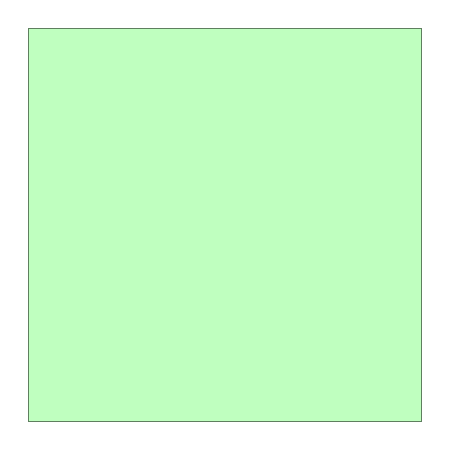
\begin{tikzpicture}
    \filldraw[initialcellstyle] 
    (0,0)
    rectangle
    +(\celldimension, -\celldimension);
  \end{tikzpicture}
}

\savebox{\finalcell}{
  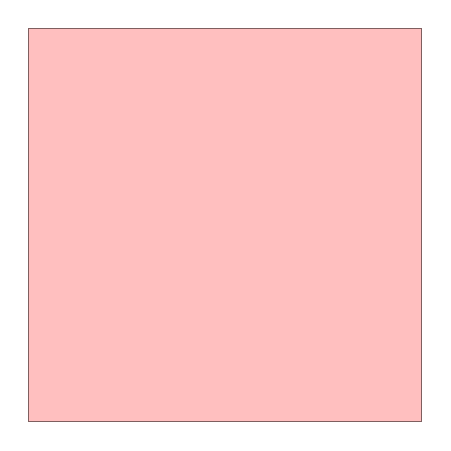
\begin{tikzpicture}
    \filldraw[finalcellstyle] 
    (0,0)
    rectangle
    +(\celldimension, -\celldimension);
  \end{tikzpicture}
}
\PRODUCEDOCUMENT
\end{document}

%%% Local Variables: 
%%% mode: latex
%%% TeX-master: t
%%% End: 
